\newpage
\chapter{Løsninger og mindste kvadraters løsninger af lineære ligningssystemer}
([P] 1.2, 5.2, 7.2.10-7.2.13, 8.2.9)

\section*{Disposition}
\begin{enumerate}
	\item Lineær Ligningssystem
	\item \sout{Rækkeækvivalens}
	\item ERO'er
	\item REF \& RREF
	\item Konsistens i Ligningssystemer
	\item Mindste Kvadraters Løsninger
\end{enumerate}

\section{Lineære Ligningssystemer}

\kbox{Eventuelt finde bevis der passer til lineære liningssystemer og måske
	definere hvad søjlerum og nulrum er.}

\subsection{Definition}
Et lineært ligningssystem er et system af $m$ ligninger i $n$ ubekendte, hvor 
disse kan skrives som:

\begin{align*}
	a_{1,1}x_1 + \dots + a_{1,n}x_n & = b_1\\
									& \vdots \\
	a_{m,1}x_1 + \dots + a_{m,n}x_n & = b_m
\end{align*}
Et sådan system kan også opstilles på matrix form, hvor $A$ er en matrix, $x$
og $b$ er vektorer:
\[
	Ax = b
\]
Systemet løses ved at indsætte $c_1, \dots, c_n$ på $x$ plads, så begge sider
af ligheden af den samme, altså er vektoren $c$ en del af løsningsmængden.

\section{Rækkeækvivalens}

Hvis løsningsmængden for et ligningssystem $Ax = b$ og $Cx = d$ er ens, altså
de har de samme $x$, kan $A$ og $C$ siges at være rækkeækvivalente.
Sammenhængen mellem $A$ og $C$ vil da være at der er blevet benyttet en række
\textit{ERO'er} på $A$ for at danne $C$.

\subsection{ERO'er}
Der er 3 elementære rækkeoperationer, som kan bruges til at manipulere med
ligningssystemer.

\begin{enumerate}
	\item $R_i \Leftrightarrow R_j$: byt den $i$'te og den $j$'te ligning.
	\item $R_i \Rightarrow sR_i$: gang den $i$'te ligning med $s \in 
		\mathbb{F} \bs \{0\}$
	\item $R_i \Rightarrow R_i+tR_j$: addér $t$ gange $R_j$ til $R_i$ når $t 
		\in \mathbb{F}, j \not= i$.
\end{enumerate}


\section{REF \& RREF}
\subsection{REF}
Række Echelon From, er en bestemt form, som en matrix kan komme på. Dette ved 
hjælp af \textit{ERO'er}. Formen er som følger:

\begin{enumerate}
	\item Nulrækker, ligger nederst i matricen.
	\item Den første ikke-nulindgang i en række er 1 og ligger til højre for
		den første ikke-nulindgang i rækken ovenover.
\end{enumerate}
Den første ikke-nulindgang på en række i en REF-matrix, kaldes en 
\textit{pivot}.

\subsection{RREF}
En matrix er på RREF (Reduceret Række Echelon Form), hvis den er på REF, og 
alle søjler som indeholder en pivot har 0 på alle andre indgange.

\section{Konsistens i Ligningssystemer}
\begin{lemma}{2.2.4}
	Lad $A \in \mat_{m,n}$. Skriv $A = [\vec{a_1}, \dotsc, \vec{a_n}]$ i 
	søjleform. 
	
	Betragt da ligningssystemet $A\vec{x} = \vec{b}$, hvor $b \in 
	\mathbb{F}^{m \times 1}$.

	Systemet er konsistent (har en løsning) $\Leftrightarrow b \in 
	\spn(\vec{a_1}, \dotsc, \vec{a_n})$.
\end{lemma}


\section{Mindste Kvadraters Løsninger}
En mindste kvadraters løsning er hvor man finder den bedst mulige løsning, til
et ligningssystem med flere ligninger end ubekendte. Generelt kan det beskrives
som $Ax=b$ hvor $A \in Mat_{m,n}(\mathbb{R})$ med $m>n$. 

Generelt kan det ikke forventes at man kan finde et $x \in \mathbb{R}^n$ som
løser ligningssystemet, hvilket gør at man leder efter et $z \in \mathbb{R}^n$
som får $Az$ til at være tættest på $b \in \mathbb{R}^m$.

\begin{center}
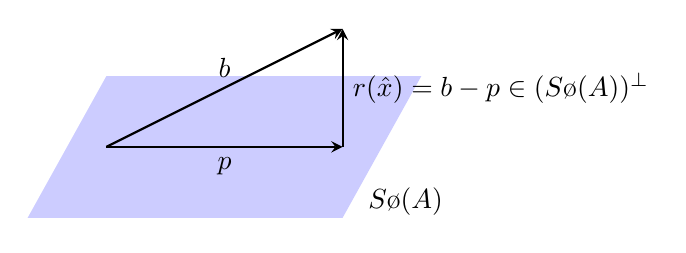
\begin{tikzpicture}
	\tikzset{>=stealth}
	\fill[blue!20] (0,0) -- (1,1.8) -- (5,1.8) -- (4,0) -- cycle;

	\node (sa) at (4.8,0.2) {$S\text{ø}(A)$};
	
	\draw[thick,->] (1,0.9) to node[below]{$p$} (4,0.9);
	\draw[thick,->] (1,0.9) to node[above]{$b$} (4,2.4);
	\draw[thick,->] (4,0.9) to node[right]{$r(\hat{x})=b-p\in 
		(S\text{ø}(A))^\bot$} (4,2.4);
\end{tikzpicture}
\end{center}


Hvis man har ovenstående ligningssystem kan man finde et residual
\[
	r(x) = b - Ax
\]
som er den ``overskydende'' afstand mellem den bedste løsning og punkterne. Vi
søger derfor at finde den den mindste længde, $\norm{r(x)}$, for residualet, hvilket
er det samme som at søge den mindst mulige løsning til $\norm{r(x)}^2$. En vektor
$\hat{x}$ der opfylder dette, siges at være en mindste kvadraters løsning for
$Ax = b$ og $p = A\hat{x}$, hvilket gør $p \in S\text{ø}(A)$, der er tættest på
$b$.

\begin{proposition}{5.2.2}
	Der er et unikt $p \in \so (A)$ som er tættest på $b$. Altså
	\[
		\norm{b-y} > \norm{b-p}
	\]
	hvor $y, p \in \so(A)$ og $y \not= p$.
\end{proposition}

\begin{bevis}
	Beviset for at $p$ er unik er som følger. Enhver vektor $b \in
	\mathbb{R}^m$ kan beskrives som
	\[
		b = p + z
	\]
	hvor $p \in \so(A)$ og $z \in (\so(A))^\bot$. Givet en vektor $y \in
	\so(A)$ forskellig fra $p$ gælder
	\[
		\norm{b-y}^2 = \norm{(b-p)+(p-y)}^2
	\]
	\begin{center}
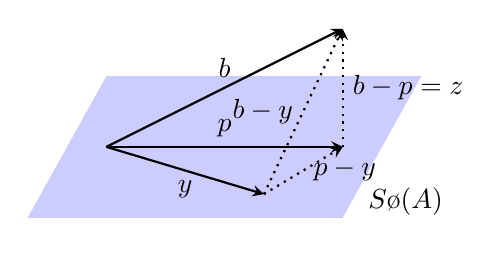
\begin{tikzpicture}
	\tikzset{>=stealth}
	\fill[blue!20] (0,0) -- (1,1.8) -- (5,1.8) -- (4,0) -- cycle;

	\node (sa) at (4.8,0.2) {$S\text{ø}(A)$};

	\coordinate (s) at (1,0.9);
	\coordinate (pE) at (4,0.9);
	\coordinate (bE) at (4,2.4);
	\coordinate (yE) at (3,0.3);
	
	\draw[thick,->] (s) to node[above]{$p$} (pE);
	\draw[thick,->] (s) to node[above]{$b$} (bE);
	\draw[thick,->,dotted] (pE) to node[right]{$b-p = z$} (bE);
	\draw[thick,->] (s) to node[below]{$y$} (yE);
	\draw[thick,->,dotted] (yE) to node[left]{$b-y$} (bE);
	\draw[thick,->,dotted] (yE) to node[right]{$p-y$} (pE);
\end{tikzpicture}
\end{center}

	da $p-y \in \so(A)$ og $b-p = z \in (\so(A))^\bot$ så får vi fra Pythagoras
	\[
		\norm{b-y}^2 = \norm{b-p}^2 + \norm{p-y}^2
	\]
	og vi kan derfor konkludere at
	\[
		\norm{b-y} > \norm{b-p}
	\]
\end{bevis}

\begin{proposition}{5.2.4}
	Systemet $A^T Ax = A^T b$ er konsistent, og $z$ er en løsning til dette 
	system, hhvis $z$ er en mindste kvadraters løsning til $Ax =  b$.
\end{proposition}

\begin{bevis}
	\begin{align*}
		Az = p &\Lra b - Az \in (S\text{ø}(A))^\bot 
				& \text{fordi }p = P_{S\text{ø}(A)}(b) \\
			& \Lra b - Az \in N(A^T) & \text{Sætning 5.1.16} \\
			& \Lra A^T (b - Az) = 0 \\
			& \Lra A^T b = A^T Az
	\end{align*}
\end{bevis}


